\documentclass[12pt,a4paper]{article}
\usepackage{amsmath, amssymb, geometry}
\geometry{margin=1in}
\usepackage{siunitx}
\usepackage{bm}
\usepackage{hyperref}
\usepackage{url}
\usepackage{graphicx}

\title{Week 06 Assignment Based on Book Computer Vision by Richard Szeliski, Second Edition, Chapter 8}
\author{Bishwash Khanal, \texttt{bishwash.b.khanal@student.jyu.fi}}
\date{October 19, 2025}

\begin{document}

\maketitle

\section{2D match move/augmented reality}
Replace silver colored Honda Civic hatchback car in the given video clip (the very first car when video clip starts to play) with a different 
colored and model car of your liking (e.g., White Toyota RAV4).

Link to video clip: \url{https://drive.google.com/file/d/1p2g68kxvXnez9yc2nhD6XJ0aGTx2tyRX/view?usp=sharing}

Key steps:
\begin{enumerate}
    \item Outline a figure or picture on the page with a rectangle, i.e., draw over the four sides as they appear in the image (in this case, 
    image of original car in video which you should replace).
    \item Match features in this area with each new image frame.
    \item Replace the original image with an "advertising” insert, warping the new image with the appropriate homography.
\end{enumerate}

Submit your code (Python Notebook) showing all intermediate steps which takes provided video clip as input and produces final 
video clip with your replaced car. Also, submit your final video.

\textbf{Notebook:} \href{https://colab.research.google.com/drive/1Yzvp8Du_17CSvvjYdGxLVsR-M0sM8QJU?usp=sharing}{Assignment\_Week6\_Q1.ipynb (Google Colab)} - 
\href{https://github.com/bkhanal-11/ties411_cvip_jyu/blob/master/assignment6/src/Assignment_Week6_Q1.ipynb}{(GitHub)}

\textbf{Final video:} \url{https://drive.google.com/file/d/1Ti-yIweh4527cvQm2LG_Q5UlFQ189jYp/view?usp=sharing}

\section{Stitching overlapping images}
You are given five overlapping images at this link: \url{https://drive.google.com/drive/folders/1RRKGSiRIpYTK2KTNZxPMZHzf6Cwg-M-v?usp=share_link}

You are supposed to stitch all images given above and generate a final image which looks like 
this: \url{https://drive.google.com/file/d/1igoXko7qtae5RxxB_ddpY7TKVaX2vc1d/view?usp=sharing}

Follow these steps:
\begin{enumerate}
    \item Arrange pictures such that adjacent pictures have atleast 40\% overlap. Order the pictures from left to right.
    \item Generate SIFT features among images.
    \item Establish correspondence between features.
    \item Apply RANSAC (Random Sampling and Consensus) to get rid of outliers.
    \item Generate initial estimate of Homography using inlier correspondence points obtained in step 4 (RANSAC step).
    \item Refine the Homography estimate using Levenberg- Marquardt optimization.
    \item Repeat the above steps for each of the adjacent image pairs.
    \item After obtaining Homographies for each of the picture pairs, get the homographies with respect to the central image
    \item Project all images (using inverse warping) on to a blank canvas. Use bilinear interpolation
\end{enumerate}

You are welcome to use Python OpenCV library.

Submit your source code (python notebook) showing all steps indicated above which takes all overlapping images as input, 
and produces final stitched image shown in the question. Also submit final stitched image produced by your code.

\textbf{Notebook:} \href{https://colab.research.google.com/drive/1eCEGWNIpp4dDtilvpM9eyMrYHPYjlth4?usp=sharing}{Assignment\_Week6\_Q2.ipynb (Google Colab)} - 
\href{https://github.com/bkhanal-11/ties411_cvip_jyu/blob/master/assignment6/src/Assignment_Week6_Q2.ipynb}{(GitHub)}

\begin{figure}[h]
    \centering
    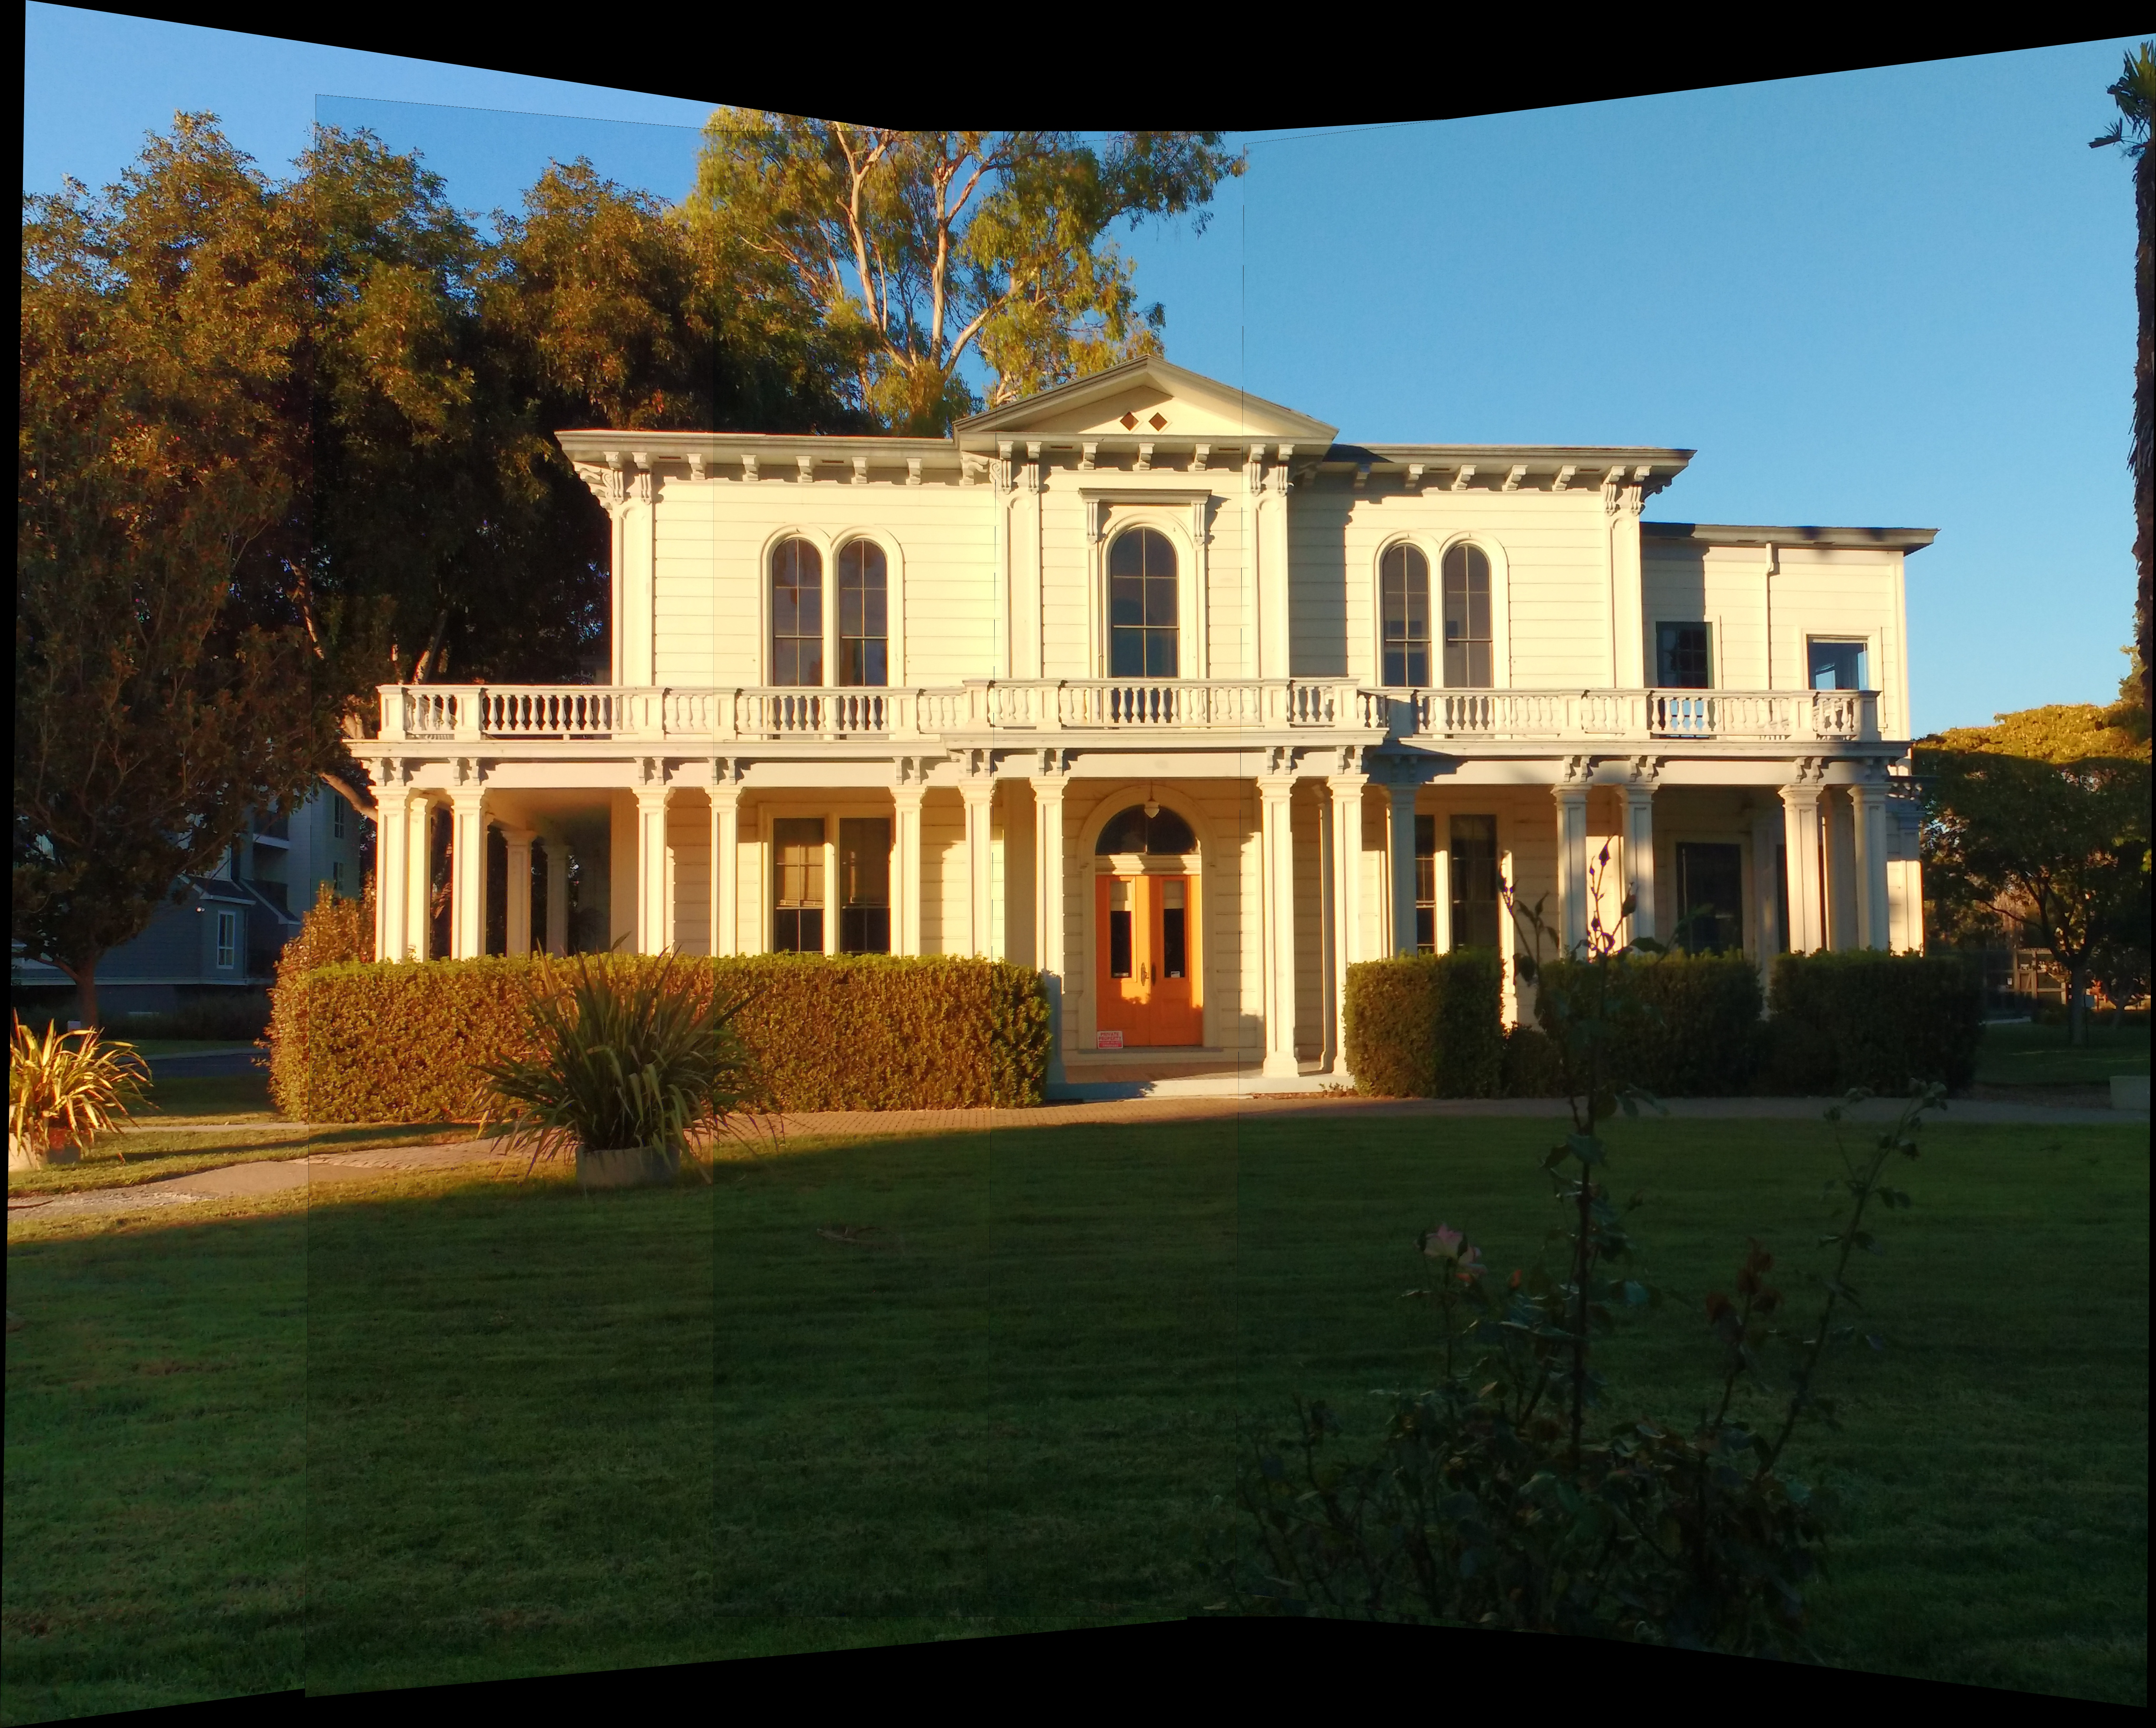
\includegraphics[width=0.95\textwidth]{src/final_panorama.jpg}
    \caption{Final panorama image}
    \label{fig:final_panorama}
\end{figure}

\end{document}
